%%%%%%%%%%%%%%%%%%%%%%%%%%%%%%%%%%%%%%%%%%%%%%%%%%%%%%%%%%%%%%%%%%%%%%
\begin{frame}[fragile]\frametitle{}
\begin{center}
{\Large Dynamic Programming}
\end{center}

		{\tiny (Ref: ``Dynamic Programming' - Bjarki Agust Guomundsson, Tomas Ken Magnusson, ``CS1101S: Programming Methodology'' - Martin Henz)}

\end{frame}

%%%%%%%%%%%%%%%%%%%%%%%%%%%%%%%%%%%%%%%%%%%%%%%%%%%%%%%%%%%%%%%%%%%%%%
\begin{frame}[fragile]{What is dynamic programming?}
    \begin{itemize}
        \item A problem solving paradigm
        \item Similar in some respects to both divide and conquer and backtracking
        \vspace{5pt}
        \item Divide and conquer recap:
            \begin{itemize}
                \item Split the problem into \textit{independent} subproblems
                \item Solve each subproblem recursively
                \item Combine the solutions to subproblems into a solution for the given problem
            \end{itemize}
        \vspace{5pt}
        \item Dynamic programming:
            \begin{itemize}
                \item Split the problem into \textit{overlapping} subproblems
                \item Solve each subproblem recursively
                \item Combine the solutions to subproblems into a solution for the given problem
                \item \textit{Don't compute the answer to the same problem more than once}
            \end{itemize}
				\item Formulation:
            \begin{itemize}
							\item Formulate the problem in terms of smaller versions of the problem (recursively)
							\item Turn this formulation into a recursive function
							\item Memoize the function (remember results that have been computed)						
            \end{itemize}
				
    \end{itemize}
		
\end{frame}

%%%%%%%%%%%%%%%%%%%%%%%%%%%%%%%%%%%%%%%%%%%%%%%%%%%%%%%%%%%%%%%%%%%%%%
\begin{frame}[fragile]
	\frametitle{Introduction}
		
			\begin{itemize}
			\item Dynamic programming is nothing but recursion + memoization
				\item Extension of recursion that further optimists time complexity by storing intermediate values of 
recursion so they don’t have to be re-computed. 
				\item The array/structure that stores these values is 
called a memo, and the process of storing them memoization. 
				\item A ``bottom up” approach uses 
``tabulation” instead of ``memoisation''. 
				\item Memoization is ``top-down'' because, like in the fib(n) 
example, you compute $fib(5)$ before looking for $fib(4)$ which is needed to compute $fib(5)$, whereas a 
bottom-up approach finds $fib(4)$ and puts it in a variable/array before using it to computer $fib(5)$ at 
all. 
				\item Tabulation is more efficient when all sub-problems must be solved at least once to get the final 
result (as in the $fib(n)$ problem) but memoization is faster otherwise because it strictly only 
computers things that need to be computed. 
			\end{itemize}
\end{frame}

%%%%%%%%%%%%%%%%%%%%%%%%%%%%%%%%%%%%%%%%%%%%%%%%%%%%%%%%%%%%%%%%%%%%%%
\begin{frame}[fragile]
	\frametitle{Difference}
		
			\begin{itemize}
				\item There’s a difference between divide and conquer (a class of algorithms) and dynamic programming 
(a technique for thinking about/approaching problems). 
\item In divide and conquer, the sub-problems 
don’t overlap. 
\item In DP, they do, and it’s optimal to cache the overlaps via memorization to optimize. 
			\end{itemize}
			
\begin{center}
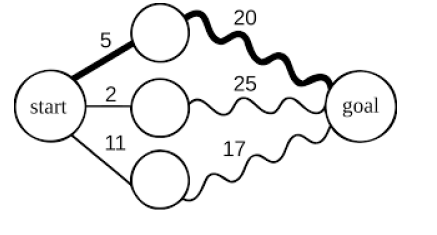
\includegraphics[width=0.5\linewidth,keepaspectratio]{dsa12}
\end{center}				
\end{frame}

% Graph styles
\tikzstyle{vertex}=[circle,fill=black!50,minimum size=15pt,inner sep=0pt, font=\small]
\tikzstyle{selected vertex} = [vertex, fill=red!24]
\tikzstyle{edge} = [draw,thick,-]
\tikzstyle{dedge} = [draw,thick,->]
\tikzstyle{weight} = [font=\scriptsize,pos=0.5]
\tikzstyle{selected edge} = [draw,line width=2pt,-,red!50]
\tikzstyle{ignored edge} = [draw,line width=5pt,-,black!20]

%%%%%%%%%%%%%%%%%%%%%%%%%%%%%%%%%%%%%%%%%%%%%%%%%%%%%%%%%%%%%%%%%%%%%%
\begin{frame}[fragile]{The Fibonacci sequence}
    \textit{The first two numbers in the Fibonacci sequence are 1 and 1. All
            other numbers in the sequence are defined as the sum of the previous two
            numbers in the sequence.}

    \begin{itemize}
        \item Task: Find the $n$th number in the Fibonacci sequence
        \item Let's solve this with dynamic programming
    \end{itemize}

    \begin{itemize}
        \item Formulate the problem in terms of smaller versions of the problem (recursively)
    \end{itemize}

    \begin{align*}
        \mathrm{fibonacci}(1) &= 1\\
        \mathrm{fibonacci}(2) &= 1\\
        \mathrm{fibonacci}(n) &= \mathrm{fibonacci}(n - 2) + \mathrm{fibonacci}(n - 1)
    \end{align*}
\end{frame}

%%%%%%%%%%%%%%%%%%%%%%%%%%%%%%%%%%%%%%%%%%%%%%%%%%%%%%%%%%%%%%%%%%%%%%
\begin{frame}[fragile]{The Fibonacci sequence}
    \begin{itemize}
        \item[2.] Turn this formulation into a recursive function
    \end{itemize}

    \begin{lstlisting}[basicstyle=\footnotesize]{cpp}
int fibonacci(int n) {
    if (n <= 2) {
        return 1;
    }

    int res = fibonacci(n - 2) + fibonacci(n - 1);

    return res;
}
    \end{lstlisting}
\end{frame}

%%%%%%%%%%%%%%%%%%%%%%%%%%%%%%%%%%%%%%%%%%%%%%%%%%%%%%%%%%%%%%%%%%%%%%
\begin{frame}[fragile]{The Fibonacci sequence}
    \begin{itemize}
        \item What is the time complexity of this? \onslide<2->{Exponential, almost $O(2^n)$}
    \end{itemize}

    \begin{figure}

        \begin{tikzpicture}

[-,thick,%
  every node/.style={shape=circle,draw,thick},%
  level distance=0.5cm,
  growth parent anchor={south}, nodes={anchor=north},
  scale=0.8,%
]
\scriptsize
\node {$fib(6)$}
  [sibling distance=5cm]
  child {node {$fib(4)$}
    [sibling distance=2cm]
    child {node {$fib(2)$}
      % [sibling distance=0.5cm]
      % % child {node {$0$}}
      % child {node {$fib(1)$}
      %   % child {node {$0$}}
      %   % child {node {$0$}}
      % }
    }
    child {node {$fib(3)$}
      [sibling distance=1cm]
      child {node {$fib(1)$}
        [sibling distance=0.5cm]
        % child {node {$0$}}
        % child {node {$0$}}
      }
      child {node {$fib(2)$}
        % [sibling distance=0.5cm]
        % % child {node {$0$}}
        % child {node {$fib(1)$}
        %   % child {node {$0$}}
        %   % child {node {$0$}}
        % }
      }
    }
  }
  child {node {$fib(5)$}
    [sibling distance=3cm]
    child {node {$fib(3)$}
      [sibling distance=1cm]
      child {node {$fib(1)$}
        [sibling distance=0.5cm]
        % child {node {$0$}}
        % child {node {$0$}}
      }
      child {node {$fib(2)$}
        % [sibling distance=0.5cm]
        % % child {node {$0$}}
        % child {node {$fib(1)$}
        %   % child {node {$0$}}
        %   % child {node {$0$}}
        % }
      }
    }
    child {node {$fib(4)$}
      [sibling distance=2cm]
      child {node {$fib(2)$}
        % [sibling distance=0.5cm]
        % % child {node {$0$}}
        % child {node {$fib(1)$}
        %   % child {node {$0$}}
        %   % child {node {$0$}}
        % }
      }
      child {node {$fib(3)$}
        [sibling distance=1cm]
        child {node {$fib(1)$}
          [sibling distance=0.5cm]
          % child {node {$0$}}
          % child {node {$0$}}
        }
        child {node {$fib(2)$}
          % [sibling distance=0.5cm]
          % % child {node {$0$}}
          % child {node {$fib(1)$}
          %   % child {node {$0$}}
          %   % child {node {$0$}}
          % }
        }
      }
    }
  };
        \end{tikzpicture}

% \tikzset{
%   treenode/.style = {align=center, inner sep=0pt, text centered,
%     font=\sffamily},
%   vertex/.style = {treenode, circle, white, font=\sffamily\bfseries\tiny, draw=white,
%     text width=1.8em},% arbre rouge noir, noeud noir
% }
% 
% \begin{tikzpicture}
%     [->,>=stealth',level/.style={sibling distance = 5cm/#1,
%   level distance = 1.8cm},scale=0.8] 
%   \node [vertex] {fib(10)}
%     child{ node [vertex] {fib(8)}
%             child{ node [vertex] {fib(6)} 
%                 child{ node [vertex] {fib(4)} }
%                 child{ node [vertex] {fib(5)}}
%             }
%             child{ node [vertex] {fib(7)}
%                             child{ node [vertex] {fib(5)}}
%                             child{ node [vertex] {fib(6)}}
%             }
%     }
%     child{ node [vertex] {fib(9)}
%         child{ node [vertex] {fib(7)} 
%             child{
%                 node [vertex] {fib(5)}
%                     child { node [vertex] {fib(3)} }
%                     child { node [vertex] {fib(4)} }
%                 }
%             child{ node [vertex] {fib(6)}
%             }
%             }
%             child{ node [vertex] {fib(8)}
% 							child{ node [vertex] {49}}
% 							% child{ node [vertex] {}}
%             }
% 		}
% ; 
% \end{tikzpicture}
            \end{figure}

\end{frame}

%%%%%%%%%%%%%%%%%%%%%%%%%%%%%%%%%%%%%%%%%%%%%%%%%%%%%%%%%%%%%%%%%%%%%%
\begin{frame}[fragile]{The Fibonacci sequence}
    \begin{itemize}
        \item[3.] Memoize the function (remember results that have been computed)
    \end{itemize}

    \begin{lstlisting}[basicstyle=\footnotesize]{cpp}
map<int, int> mem;

int fibonacci(int n) {
    if (n <= 2) {
        return 1;
    }

    if (mem.find(n) != mem.end()) {
        return mem[n];
    }

    int res = fibonacci(n - 2) + fibonacci(n - 1);

    mem[n] = res;
    return res;
}
    \end{lstlisting}

\end{frame}

%%%%%%%%%%%%%%%%%%%%%%%%%%%%%%%%%%%%%%%%%%%%%%%%%%%%%%%%%%%%%%%%%%%%%%
\begin{frame}[fragile]{The Fibonacci sequence}

    \begin{lstlisting}[basicstyle=\footnotesize]{cpp}
int mem[1000];
for (int i = 0; i < 1000; i++)
    mem[i] = -1;

int fibonacci(int n) {
    if (n <= 2) {
        return 1;
    }

    if (mem[n] != -1) {
        return mem[n];
    }

    int res = fibonacci(n - 2) + fibonacci(n - 1);

    mem[n] = res;
    return res;
}
    \end{lstlisting}

\end{frame}

%%%%%%%%%%%%%%%%%%%%%%%%%%%%%%%%%%%%%%%%%%%%%%%%%%%%%%%%%%%%%%%%%%%%%%
\begin{frame}[fragile]{The Fibonacci sequence}
    \begin{itemize}
        \item What is the time complexity now?
        \item We have $n$ possible inputs to the function: $1$, $2$, \ldots, $n$.
        \item Each input will either:
            \begin{itemize}
                \item be computed, and the result saved
                \item be returned from the memory
            \end{itemize}
        \item Each input will be computed at most once
        \item Time complexity is $O(n \times f)$, where $f$ is the time complexity of computing an input if we assume that the recursive calls are returned directly from memory ($O(1)$)
        \item Since we're only doing constant amount of work to compute the answer to an input, $f = O(1)$
        \item Total time complexity is $O(n)$
    \end{itemize}
\end{frame}

%%%%%%%%%%%%%%%%%%%%%%%%%%%%%%%%%%%%%%%%%%%%%%%%%%%%%%%%%%%%%%%%%%%%%%
\begin{frame}{Egg Dropping Puzzle}
\begin{block}{Given}
$n$ eggs, building with $k$ floors
\end{block}

\begin{block}{Wanted}
Smallest number of egg dropping experiments required
to find out in all cases,
which floors an egg can be safely dropped from
\end{block}

\end{frame}

%%%%%%%%%%%%%%%%%%%%%%%%%%%%%%%%%%%%%%%%%%%%%%%%%%%%%%%%%%%%%%%%%%%%%%
\begin{frame}{Assumptions}

\begin{itemize}
\item An egg that survives a fall can be used again.
\item A broken egg must be discarded.
\item The effect of a fall is the same for all eggs.
\item If an egg breaks when dropped, 
then it would break if dropped from a higher floor.
\item If an egg survives a fall then it would survive a shorter fall.
\item A first-floor drop may break eggs, and eggs may survive
a drop from the highest floor.
\end{itemize}

\end{frame}


%%%%%%%%%%%%%%%%%%%%%%%%%%%%%%%%%%%%%%%%%%%%%%%%%%%%%%%%%%%%%%%%%%%%%%
\begin{frame}{Special Case: One Egg}

\begin{block}{Number of eggs $= 1$, number of floors $= 21$}
We need at most 21 experiments
\end{block}

\end{frame}


%%%%%%%%%%%%%%%%%%%%%%%%%%%%%%%%%%%%%%%%%%%%%%%%%%%%%%%%%%%%%%%%%%%%%%
\begin{frame}{Special Case: Two Eggs}

\begin{block}{Animated scenario}
\href{http://archive.ite.journal.informs.org/Vol4No1/Sniedovich/index.php}{click here}
\end{block}

\end{frame}


%%%%%%%%%%%%%%%%%%%%%%%%%%%%%%%%%%%%%%%%%%%%%%%%%%%%%%%%%%%%%%%%%%%%%%
\begin{frame}{Observations}

\begin{block}{Sub-tasks}
At each point in time, we have a number of eggs $n$ available 
and a number of floors $k$ to check
\end{block}

\begin{block}{Contiguous floors to check}
The height of the floors does not matter. At each point in time
we need to check a certain number of contiguous floors, say from
$10$ to $14$.
\end{block}

\begin{block}{Height does not matter}
Checking $10$ to $14$ is the same as checking 
$20$ to $24$.
\end{block}

\end{frame}

%%%%%%%%%%%%%%%%%%%%%%%%%%%%%%%%%%%%%%%%%%%%%%%%%%%%%%%%%%%%%%%%%%%%%%
\begin{frame}[fragile]{A simple algorithm}
\begin{lstlisting}
function eggDrop(n, k) {
   if (k =< 1 || n === 1) {
      return k;
   } else {
      var min = large_constant;
      var x = 1;
      var res = undefined;
      while (x <= k) {
         res = max(eggDrop(n-1, x-1),
                   eggDrop(n, k-x));
         if (res < min) min = res;
         x = x + 1;
      }
      return min + 1;
}  }
\end{lstlisting}
\end{frame}


%%%%%%%%%%%%%%%%%%%%%%%%%%%%%%%%%%%%%%%%%%%%%%%%%%%%%%%%%%%%%%%%%%%%%%
\begin{frame}[fragile]{Solution Idea}

\begin{block}{Observation}
We compute \lstinline{eggDrop(i,j)} over and over again.
\end{block}


\begin{block}{Remember results in a table}
Allocate a 2-D table \lstinline{eggFloor} that remembers
the results; after computing \lstinline{s = eggDrop(i,j)},
remember \lstinline{s} in a table.
\end{block}

\begin{lstlisting}
eggDrop[i][j] = s;
\end{lstlisting}

\end{frame}

%%%%%%%%%%%%%%%%%%%%%%%%%%%%%%%%%%%%%%%%%%%%%%%%%%%%%%%%%%%%%%%%%%%%%%
\begin{frame}[fragile]{Maximum sum}

    \begin{itemize}
\item Given an array $\mathrm{arr}[0]$, $\mathrm{arr}[1]$, \ldots, $\mathrm{arr}[n-1]$ of integers, find the interval with the highest sum
    \end{itemize}

    \begin{center}
        \begin{tabular}{|c|c|c|c|c|c|c|}
            \hline
            % -15 & \color<2->{vhilight}{8} & \color<2->{vhilight}{-2} & \color<2->{vhilight}{1} & \color<2->{vhilight}{0} & \color<2->{vhilight}{6} & -3 \\
						-15 & 8 & -2 & 1 & 0 & 6 & -3 \\
            \hline
        \end{tabular}
    \end{center}

    \begin{itemize}
        \item The maximum sum of an interval in this array is $13$

        \item But how do we solve this in general?
            \begin{itemize}
        \item Easy to loop through all $\approx n^2$ intervals, and calculate their sums, but that is $O(n^3)$
        \item We could use our static range sum trick to get this down to $O(n^2)$
        \item Can we do better with dynamic programming?
            \end{itemize}
    \end{itemize}

\end{frame}

%%%%%%%%%%%%%%%%%%%%%%%%%%%%%%%%%%%%%%%%%%%%%%%%%%%%%%%%%%%%%%%%%%%%%%
\begin{frame}[fragile]{Maximum sum}

    \begin{itemize}
        \item First step is to formulate this recursively
        \item Let $\mathrm{max\_{}sum}(i)$ be the maximum sum interval in the range $0,\ldots,i$
        \item Base case: $\mathrm{max\_{}sum}(0) = \mathrm{max}(0, arr[0])$
        \item What about $\mathrm{max\_{}sum}(i)$?
        \item What does $\mathrm{max\_{}sum}(i-1)$ return?
        \item Is it possible to combine solutions to subproblems with smaller $i$ into a solution for $i$?
        \item At least it's not obvious...
    \end{itemize}

\end{frame}

%%%%%%%%%%%%%%%%%%%%%%%%%%%%%%%%%%%%%%%%%%%%%%%%%%%%%%%%%%%%%%%%%%%%%%
\begin{frame}[fragile]{Maximum sum}

    \begin{itemize}
        \item Let's try changing perspective
    \item Let $\mathrm{max\_{}sum}(i)$ be the maximum sum interval in the range $0,\ldots,i$, \textit{that ends at $i$}
        \item Base case: $\mathrm{max\_{}sum}(0) = arr[0]$
    \item $\mathrm{max\_{}sum}(i) = \mathrm{max}(arr[i], arr[i] + \mathrm{max\_{}sum}(i - 1))$
        \item Then the answer is just $\mathrm{max}_{\ 0 \leq i < n}\ \{\ \mathrm{max\_{}sum}(i)\ \}$
    \end{itemize}

\end{frame}

%%%%%%%%%%%%%%%%%%%%%%%%%%%%%%%%%%%%%%%%%%%%%%%%%%%%%%%%%%%%%%%%%%%%%%
\begin{frame}[fragile]{Maximum sum}
    \begin{itemize}
        \item Next step is to turn this into a function
    \end{itemize}

    \begin{lstlisting}{cpp}
int arr[1000];

int max_sum(int i) {
    if (i == 0) {
        return arr[i];
    }

    int res = max(arr[i], arr[i] + max_sum(i - 1));

    return res;
}
    \end{lstlisting}
\end{frame}

%%%%%%%%%%%%%%%%%%%%%%%%%%%%%%%%%%%%%%%%%%%%%%%%%%%%%%%%%%%%%%%%%%%%%%
\begin{frame}[fragile]{Maximum sum}
    \begin{itemize}
        \item Final step is to memoize the function
    \end{itemize}

    \begin{lstlisting}[basicstyle=\scriptsize]{cpp}
int arr[1000];
int mem[1000];
bool comp[1000];
memset(comp, 0, sizeof(comp));

int max_sum(int i) {
    if (i == 0) {
        return arr[i];
    }
    if (comp[i]) {
        return mem[i];
    }

    int res = max(arr[i], arr[i] + max_sum(i - 1));

    mem[i] = res;
    comp[i] = true;
    return res;
}
    \end{lstlisting}
\end{frame}

%%%%%%%%%%%%%%%%%%%%%%%%%%%%%%%%%%%%%%%%%%%%%%%%%%%%%%%%%%%%%%%%%%%%%%
\begin{frame}[fragile]{Maximum sum}
    \begin{itemize}
        \item Then the answer is just the maximum over all interval ends
    \end{itemize}

    \begin{lstlisting}{cpp}
int maximum = 0;
for (int i = 0; i < n; i++) {
    maximum = max(maximum, best_sum(i));
}

printf("%d\n", maximum);
    \end{lstlisting}
\end{frame}

%%%%%%%%%%%%%%%%%%%%%%%%%%%%%%%%%%%%%%%%%%%%%%%%%%%%%%%%%%%%%%%%%%%%%%
\begin{frame}[fragile]{Maximum sum}
    \begin{itemize}
        \item If you want to find the maximum sum interval in multiple arrays, remember to clear the memory in between
        \item What about time complexity?
        \item There are $n$ possible inputs to the function
        \item Each input is processed in $O(1)$ time, assuming recursive calls are $O(1)$
        \item Time complexity is $O(n)$
    \end{itemize}
\end{frame}

%%%%%%%%%%%%%%%%%%%%%%%%%%%%%%%%%%%%%%%%%%%%%%%%%%%%%%%%%%%%%%%%%%%%%%
\begin{frame}[fragile]{Coin change}

    \begin{itemize}
\item Given an array of coin denominations $d_0$, $d_2$, \ldots, $d_{n-1}$,
            and some amount $x$: What is minimum number of coins needed to
            represent the value $x$?

        \item Remember the greedy algorithm for Coin change?
        \item It didn't always give the optimal solution, and sometimes it didn't even give a solution at all...

        \item What about dynamic programming?
    \end{itemize}
\end{frame}

%%%%%%%%%%%%%%%%%%%%%%%%%%%%%%%%%%%%%%%%%%%%%%%%%%%%%%%%%%%%%%%%%%%%%%
\begin{frame}[fragile]{Coin change}
    \begin{itemize}
        \item First step: formulate the problem recursively
\item Let $\mathrm{opt}(i,x)$ denote the minimum number of coins needed to represent the value $x$ if we're only allowed to use the coin denominations $d_0$, \ldots, $d_i$
        \item Base case: $\mathrm{opt}(i,x) = \infty$ if $x < 0$
        \item Base case: $\mathrm{opt}(i,0) = 0$
        \item Base case: $\mathrm{opt}(-1,x) = \infty$
\item $\mathrm{opt}(i,x) = \mathrm{min} \left\{
	\begin{array}{l}
        1 + \mathrm{opt}(i, x - d_i) \\
        \mathrm{opt}(i-1, x)
	\end{array}
\right.$
    \end{itemize}
\end{frame}

%%%%%%%%%%%%%%%%%%%%%%%%%%%%%%%%%%%%%%%%%%%%%%%%%%%%%%%%%%%%%%%%%%%%%%
\begin{frame}[fragile]{Coin change}
    \begin{lstlisting}[basicstyle=\footnotesize]{cpp}
int INF = 100000;
int d[10];

int opt(int i, int x) {
    if (x < 0) return INF;
    if (x == 0) return 0;
    if (i == -1) return INF;

    int res = INF;
    res = min(res, 1 + opt(i, x - d[i]));
    res = min(res, opt(i - 1, x));

    return res;
}
    \end{lstlisting}
\end{frame}

%%%%%%%%%%%%%%%%%%%%%%%%%%%%%%%%%%%%%%%%%%%%%%%%%%%%%%%%%%%%%%%%%%%%%%
\begin{frame}[fragile]{Coin change}
    \begin{lstlisting}[basicstyle=\footnotesize]{cpp}
int INF = 100000;
int d[10];
int mem[10][10000];
memset(mem, -1, sizeof(mem));

int opt(int i, int x) {
    if (x < 0) return INF;
    if (x == 0) return 0;
    if (i == -1) return INF;

    if (mem[i][x] != -1) return mem[i][x];

    int res = INF;
    res = min(res, 1 + opt(i, x - d[i]));
    res = min(res, opt(i - 1, x));

    mem[i][x] = res;
    return res;
}
    \end{lstlisting}
\end{frame}

%%%%%%%%%%%%%%%%%%%%%%%%%%%%%%%%%%%%%%%%%%%%%%%%%%%%%%%%%%%%%%%%%%%%%%
\begin{frame}[fragile]{Coin change}
    \begin{itemize}
        \item Time complexity?
        \item Number of possible inputs are $n \times x$
        \item Each input will be processed in $O(1)$ time, assuming recursive calls are constant
        \item Total time complexity is $O(n\times x)$
    \end{itemize}
\end{frame}

%%%%%%%%%%%%%%%%%%%%%%%%%%%%%%%%%%%%%%%%%%%%%%%%%%%%%%%%%%%%%%%%%%%%%%
\begin{frame}[fragile]{Coin change}
    \begin{itemize}
        \item How do we know which coins the optimal solution used?
        \item We can store backpointers, or some extra information, to trace backwards through the states
        \item See example...
    \end{itemize}
\end{frame}

%%%%%%%%%%%%%%%%%%%%%%%%%%%%%%%%%%%%%%%%%%%%%%%%%%%%%%%%%%%%%%%%%%%%%%
\begin{frame}[fragile]{Longest increasing subsequence}
    \begin{itemize}
\item Given an array $a[0]$, $a[1]$, \ldots, $a[n-1]$ of integers, what is the length of the longest increasing subsequence?
\item First, what is a subsequence?
\item If we delete zero or more elements from $a$, then we have a subsequence of $a$
\item Example: $a = [5,1,8,1,9,2]$
\item $[5,8,9]$ is a subsequence
\item $[1,1]$ is a subsequence
\item $[5,1,8,1,9,2]$ is a subsequence
\item $[]$ is a subsequence
\item $[8,5]$ is \textbf{not} a subsequence
\item $[10]$ is \textbf{not} a subsequence
    \end{itemize}
\end{frame}

%%%%%%%%%%%%%%%%%%%%%%%%%%%%%%%%%%%%%%%%%%%%%%%%%%%%%%%%%%%%%%%%%%%%%%
\begin{frame}[fragile]{Longest increasing subsequence}
    \begin{itemize}
\item Given an array $a[0]$, $a[1]$, \ldots, $a[n-1]$ of integers, what is the length of the longest increasing subsequence?
\item An increasing subsequence of $a$ is a subsequence of $a$ such that the elements are in (strictly) increasing order
\item $[5,8,9]$ and $[1,8,9]$ are the longest increasing subsequences of $a = [5,1,8,1,9,2]$
\item How do we compute the length of the longest increasing subsequence?
\item There are $2^n$ subsequences, so we can go through all of them
\item That would result in an $O(n2^n)$ algorithm, which can only handle $n\leq 23$
\item What about dynamic programming?

    \end{itemize}
\end{frame}

%%%%%%%%%%%%%%%%%%%%%%%%%%%%%%%%%%%%%%%%%%%%%%%%%%%%%%%%%%%%%%%%%%%%%%
\begin{frame}[fragile]{Longest increasing subsequence}
    \begin{itemize}
\item Let $\mathrm{lis}(i)$ denote the length of the longest increasing subsequence of the array $a[0]$, $\ldots$, $a[i]$
\item Base case: $\mathrm{lis}(0) = 1$
\item What about $\mathrm{lis}(i)$?
\item We have the same issue as in the maximum sum problem, so let's try changing perspective
    \end{itemize}
\end{frame}

%%%%%%%%%%%%%%%%%%%%%%%%%%%%%%%%%%%%%%%%%%%%%%%%%%%%%%%%%%%%%%%%%%%%%%
\begin{frame}[fragile]{Longest increasing subsequence}
    \begin{itemize}
\item Let $\mathrm{lis}(i)$ denote the length of the longest increasing subsequence of the array $a[0]$, $\ldots$, $a[i]$, \textit{that ends at $i$}
\item Base case: we don't need one
\item $\mathrm{lis}(i) = \mathrm{max}(1, \mathrm{max}_{j \textrm{ s.t. } a[j] < a[i]} \{ 1 + \mathrm{lis}(j) \})$
    \end{itemize}
\end{frame}

%%%%%%%%%%%%%%%%%%%%%%%%%%%%%%%%%%%%%%%%%%%%%%%%%%%%%%%%%%%%%%%%%%%%%%
\begin{frame}[fragile]{Longest increasing subsequence}
    \begin{lstlisting}[basicstyle=\footnotesize]{cpp}
int a[1000];
int mem[1000];
memset(mem, -1, sizeof(mem));

int lis(int i) {
    if (mem[i] != -1) {
        return mem[i];
    }

    int res = 1;
    for (int j = 0; j < i; j++) {
        if (a[j] < a[i]) {
            res = max(res, 1 + lis(j));
        }
    }

    mem[i] = res;
    return res;
}
    \end{lstlisting}
\end{frame}

%%%%%%%%%%%%%%%%%%%%%%%%%%%%%%%%%%%%%%%%%%%%%%%%%%%%%%%%%%%%%%%%%%%%%%
\begin{frame}[fragile]{Longest increasing subsequence}

    \begin{itemize}
        \item And then the longest increasing subsequence can be found by checking all endpoints:
    \end{itemize}

    \begin{lstlisting}{cpp}
int mx = 0;
for (int i = 0; i < n; i++) {
    mx = max(mx, lis(i));
}

printf("%d\n", mx);
    \end{lstlisting}
\end{frame}

%%%%%%%%%%%%%%%%%%%%%%%%%%%%%%%%%%%%%%%%%%%%%%%%%%%%%%%%%%%%%%%%%%%%%%
\begin{frame}[fragile]{Longest increasing subsequence}
    \begin{itemize}
        \item Time complexity?
        \item There are $n$ possible inputs
        \item Each input is computed in $O(n)$ time, assuming recursive calls are $O(1)$
        \item Total time complexity is $O(n^2)$
        \item This will be fast enough for $n \leq 10\ 000$, much better than the brute force method!
    \end{itemize}
\end{frame}


%%%%%%%%%%%%%%%%%%%%%%%%%%%%%%%%%%%%%%%%%%%%%%%%%%%%%%%%%%%%%%%%%%%%%%
\begin{frame}[fragile]{Longest common subsequence}
    \begin{itemize}
\item Given two strings (or arrays of integers) $a[0]$, \ldots, $a[n-1]$ and $b[0]$, \ldots, $b[m-1]$, find the length of the longest subsequence that they have in common.
\item $a = $\texttt{"b\underline{an}an\underline{inn}"}
\item $b = $\texttt{"k\underline{anin}a\underline{n}"}
\item The longest common subsequence of $a$ and $b$, \texttt{"aninn"}, has length 5
    \end{itemize}
\end{frame}

%%%%%%%%%%%%%%%%%%%%%%%%%%%%%%%%%%%%%%%%%%%%%%%%%%%%%%%%%%%%%%%%%%%%%%
\begin{frame}[fragile]{Longest common subsequence}
    \begin{itemize}
\item Let $\mathrm{lcs}(i, j)$ be the length of the longest common subsequence of the strings $a[0]$, \ldots, $a[i]$ and $b[0]$, \ldots, $b[j]$
\item Base case: $\mathrm{lcs}(-1, j) = 0$
\item Base case: $\mathrm{lcs}(i, -1) = 0$
\item $\mathrm{lcs}(i, j) = \mathrm{max} \left\{
	\begin{array}{ll}
        \mathrm{lcs}(i,j-1) & \\
        \mathrm{lcs}(i-1,j) & \\
        1 + \mathrm{lcs}(i-1,j-1) & \textrm{if } a[i] = b[j] \\
	\end{array}
\right.$
    \end{itemize}
\end{frame}

%%%%%%%%%%%%%%%%%%%%%%%%%%%%%%%%%%%%%%%%%%%%%%%%%%%%%%%%%%%%%%%%%%%%%%
\begin{frame}[fragile]{Longest common subsequence}
    \begin{lstlisting}[basicstyle=\scriptsize]{cpp}
string a = "bananinn",
       b = "kaninan";
int mem[1000][1000];
memset(mem, -1, sizeof(mem));

int lcs(int i, int j) {
    if (i == -1 || j == -1) {
        return 0;
    }
    if (mem[i][j] != -1) {
        return mem[i][j];
    }

    int res = 0;
    res = max(res, lcs(i, j - 1));
    res = max(res, lcs(i - 1, j));

    if (a[i] == b[j]) {
        res = max(res, 1 + lcs(i - 1, j - 1));
    }

    mem[i][j] = res;
    return res;
}
    \end{lstlisting}
\end{frame}

%%%%%%%%%%%%%%%%%%%%%%%%%%%%%%%%%%%%%%%%%%%%%%%%%%%%%%%%%%%%%%%%%%%%%%
\begin{frame}[fragile]{Longest common subsequence}
    \begin{itemize}
        \item Time complexity?
        \item There are $n\times m$ possible inputs
        \item Each input is processed in $O(1)$, assuming recursive calls are $O(1)$
        \item Total time complexity is $O(n\times m)$
    \end{itemize}
\end{frame}

%%%%%%%%%%%%%%%%%%%%%%%%%%%%%%%%%%%%%%%%%%%%%%%%%%%%%%%%%%%%%%%%%%%%%%
\begin{frame}[fragile]{DP over bitmasks}
    \begin{itemize}
        \item Remember the bitmask representation of subsets?
        \item Each subset of $n$ elements are mapped to an integer in the range $0$, \ldots, $2^{n} - 1$
        \item This makes it easy to do dynamic programming over subsets
    \end{itemize}
\end{frame}

%%%%%%%%%%%%%%%%%%%%%%%%%%%%%%%%%%%%%%%%%%%%%%%%%%%%%%%%%%%%%%%%%%%%%%
\begin{frame}[fragile]{Traveling salesman problem}
    \begin{itemize}
        \item We have a graph of $n$ vertices, and a cost $c_{i,j}$ between each pair of vertices $i, j$. We want to find a cycle through all vertices in the graph so that the sum of the edge costs in the cycle is minimal.
        \item This problem is NP-Hard, so there is no known deterministic polynomial time algorithm that solves it
        \item Simple to do in $O(n!)$ by going through all permutations of the vertices, but that's too slow if $n > 11$
        \item Can we go higher if we use dynamic programming?
    \end{itemize}
\end{frame}

%%%%%%%%%%%%%%%%%%%%%%%%%%%%%%%%%%%%%%%%%%%%%%%%%%%%%%%%%%%%%%%%%%%%%%
\begin{frame}[fragile]{Traveling salesman problem}
    \begin{itemize}
\item Without loss of generality, assume we start and end the cycle at vertex $0$
\item Let $\mathrm{tsp}(i, S)$ represent the cheapest way to go through all vertices in the graph and back to vertex $0$, if we're currently at vertex $i$ and we've already visited the vertices in the set $S$
\item Base case: $\mathrm{tsp}(i, \textrm{all vertices}) = c_{i,0}$
\item Otherwise $\mathrm{tsp}(i, S) = \mathrm{min}_{\ j \not\in S\ } \{\ c_{i,j} + \mathrm{tsp}(j, S \cup \{j\})\ \}$
    \end{itemize}
\end{frame}

%%%%%%%%%%%%%%%%%%%%%%%%%%%%%%%%%%%%%%%%%%%%%%%%%%%%%%%%%%%%%%%%%%%%%%
\begin{frame}[fragile]{Traveling salesman problem}
    \begin{lstlisting}[basicstyle=\scriptsize]{cpp}
const int N = 20;
const int INF = 100000000;
int c[N][N];
int mem[N][1<<N];
memset(mem, -1, sizeof(mem));

int tsp(int i, int S) {
    if (S == ((1 << N) - 1)) {
        return c[i][0];
    }
    if (mem[i][S] != -1) {
        return mem[i][S];
    }

    int res = INF;
    for (int j = 0; j < N; j++) {
        if (S & (1 << j))
            continue;

        res = min(res, c[i][j] + tsp(j, S | (1 << j)));
    }

    mem[i][S] = res;
    return res;
}
    \end{lstlisting}
\end{frame}

%%%%%%%%%%%%%%%%%%%%%%%%%%%%%%%%%%%%%%%%%%%%%%%%%%%%%%%%%%%%%%%%%%%%%%
\begin{frame}[fragile]{Traveling salesman problem}
    \begin{itemize}
\item Then the optimal solution can be found as follows:
    \end{itemize}

    \begin{lstlisting}{cpp}
printf("%d\n", tsp(0, 1<<0));
    \end{lstlisting}
\end{frame}

%%%%%%%%%%%%%%%%%%%%%%%%%%%%%%%%%%%%%%%%%%%%%%%%%%%%%%%%%%%%%%%%%%%%%%
\begin{frame}[fragile]{Traveling salesman problem}
    \begin{itemize}
        \item Time complexity?
        \item There are $n \times 2^n$ possible inputs
        \item Each input is computed in $O(n)$ assuming recursive calls are $O(1)$
        \item Total time complexity is $O(n^2 2^n)$
        \item Now $n$ can go up to about $20$
    \end{itemize}
\end{frame}

%%%%%%%%%%%%%%%%%%%%%%%%%%%%%%%%%%%%%%%%%%%%%%%%%%%%%%%%%%%%%%%%%%%%%%
\begin{frame}[fragile]
	\frametitle{Knapsack}
	
	\begin{columns}[T]
		\column{0.5\linewidth}		
			\begin{itemize}
				\item We have a weights array and a values array, where we want to choose those values which will return us 
the maximum weight sum (within the limit). 
				\item $max weight == 0$ will be the base case. 				
\item At every step, we have 2 
CHOICES:
			\begin{itemize}
				\item Include the value: Take value from $values[index] +$ move ahead 
				\item Exclude the value: Just move ahead 
			\end{itemize}
			\item We’re re-calculating a lot of states. Use memoization.
			\end{itemize}
		\column{0.5\linewidth}
\begin{lstlisting}
knapsack(weights [], values [], maxWeight = 0, index = i, memo_set = set()) 
{ 
  if(i ==  weights.length || maxWeight == 0){ 
  return  0; 
  } 
 
  //include the ith item 
  int include = v[i] + knapsack(w, v, maxWeight - weights[i], i+1); 
  // don't include 
  int exclude =  knapsack(w, v, maxWeight, i+1); 
 
  return Math.max(include, exclude); 
} 
\end{lstlisting}			
		
		
	\end{columns}		
\end{frame}

%%%%%%%%%%%%%%%%%%%%%%%%%%%%%%%%%%%%%%%%%%%%%%%%%%%%%%%%%%%%%%%%%%%%%%
\begin{frame}[fragile]
	\frametitle{Knapsack}
	

			\begin{itemize}
			\item We’re re-calculating a lot of states. Use memoization.
			\item We set the key and max value in the set, and then use that in the base case to return when that 
condition is reached. 
			\end{itemize}
			
\begin{lstlisting}
knapsack(weights [], values [], maxWeight = 0, index = i, memo_set = set()) 
{  
  if(i ==  weights.length || maxWeight == 0){ 
    return  0; 
  } 
 
  String key = maxWeight + "unique Key" + i; 
 
  // check if the key is inside this set 
  if(memo_set.containsKey(key)){ 
    return memo_set.get(key); 
  } 
 
  //include the ith item 
  int include = v[i] + knapsack(w, v, maxWeight - weights[i], i+1, set); 
  // don't include 
  int exclude =  knapsack(w, v, maxWeight, i+1, set); 
  memo_set.put(key,Math.max(op1, op2)); 
  return Math.max(include, exclude); 	
\end{lstlisting}			
		
		
\end{frame}
